\section{Diamond --- MLWFs for the valence bands}
\label{sec5:diamond}
\begin{itemize}
\item Outline: {\it Obtain MLWFs for the valence bands of diamond.}
\end{itemize}

\begin{figure}[h!]
\centering
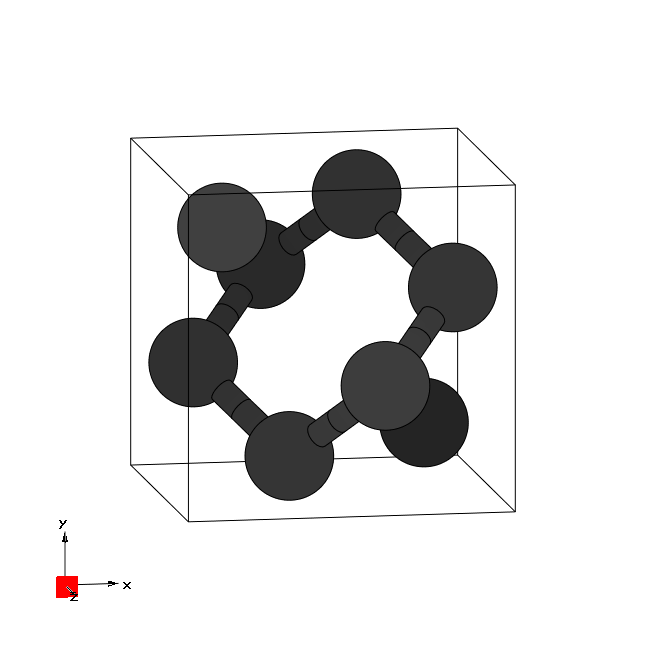
\includegraphics[width=0.25\columnwidth,trim={45pt 45pt 55pt 55pt},clip]{figure/example05/diamond.png}
\caption{Unit cell of Diamond crystal plotted with the \xcrysden{} program.}
\label{fig5.0}
\end{figure}


\begin{enumerate}
	\item {\it Run pwscf to obtain the ground state of diamond.}

	Convergence of the self-consistent field calculation in Quantum Espresso can be checked at the end of the {\tt scf.out} file. At the very end of the file one should find the line confirming that the job has finished without crashing, e.g.
	\begin{tcolorbox}[sharp corners,boxrule=0.5pt]
	{\small
	\begin{verbatim}
	=------------------------------------------------------------------------------=
	   JOB DONE.
	=------------------------------------------------------------------------------=
	\end{verbatim}
	}
	\end{tcolorbox}
	Depending on the output verbosity one may or may not find info about WALL times for the calls to the different routines. Just above this block, if present, one may find the info about the convergence of the SCF loop, such as the scf accuracy and the number of iterations to required to achieve it:  
	\begin{tcolorbox}[sharp corners,boxrule=0.5pt]
	\small{
	\begin{verbatim}
    !    total energy              =     -22.58128615 Ry
         Harris-Foulkes estimate   =     -22.58128615 Ry
         estimated scf accuracy    <          1.0E-14 Ry


         The total energy is the sum of the following terms:

         one-electron contribution =      11.69117931 Ry
         hartree contribution      =       1.57036314 Ry
         xc contribution           =      -7.58421586 Ry
         ewald contribution        =     -28.25861274 Ry

         convergence has been achieved in   9 iterations
	\end{verbatim}
	}
	\end{tcolorbox}
	\item {\it Run pwscf to obtain the Bloch states on a uniform k-point grid.}

	Similarly for the non-scf calculation one can check that the calculation has been carried out without crashing by looking at the last three line of the {\tt nscf.out} file. A useful information to check is the value of the highest eigenvalue (for insulators and semiconductors) or the value of the Fermi level (for metals). In the diamond we case, we find:
	\begin{tcolorbox}[sharp corners,boxrule=0.5pt]
	{\small
	\begin{verbatim}
	highest occupied level (ev):    19.3978
	\end{verbatim}
	}
	\end{tcolorbox}
	\item[5] {\it Run \Wannier{} to compute the MLWFs.}

	The result of the wannierisation, after 20 iterations, may be found at the end of {\tt diamond.wout} file:
	\begin{tcolorbox}[sharp corners,boxrule=0.5pt]
	\small{
	\begin{verbatim}
	 Final State
  WF centre and spread    1  ( -0.000000,  0.000000, -0.000000 )     0.58022623
  WF centre and spread    2  ( -0.806995,  0.806995,  0.000000 )     0.58022623
  WF centre and spread    3  ( -0.000000,  0.806995,  0.806995 )     0.58022623
  WF centre and spread    4  ( -0.806995, -0.000000,  0.806995 )     0.58022623
  Sum of centres and spreads ( -1.613990,  1.613990,  1.613990 )     2.32090491
 
         Spreads (Ang^2)       Omega I      =     1.954619859
        ================       Omega D      =     0.000000000
                               Omega OD     =     0.366285054
    Final Spread (Ang^2)       Omega Total  =     2.320904912
 ------------------------------------------------------------------------------
	\end{verbatim}
	}
	\end{tcolorbox}
	\item[Extra :] {\it Plot the 4 \MLWFs.} 

	The resulting 4 $\sigma$-bonding \MLWFs{} are shown in \Fig{fig5.1}
\end{enumerate}
	\begin{figure}[h!]
	\centering
 	\subfloat[\MLWF{} 1]{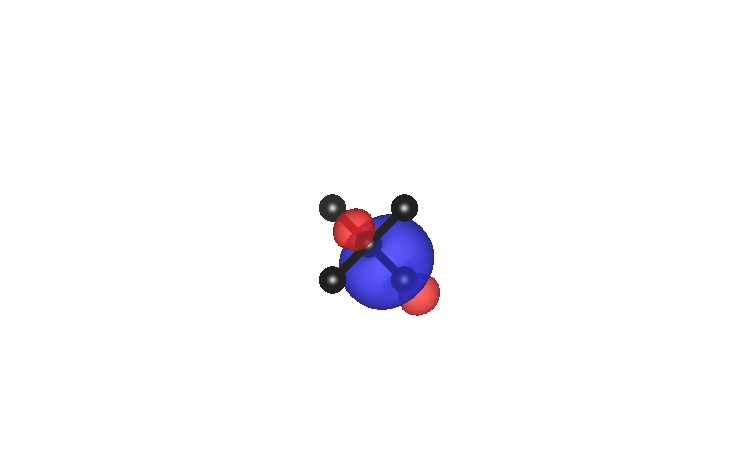
\includegraphics[width=0.2\columnwidth,trim={220pt 120pt 220pt 120pt},clip]{figure/example05/diamond_1.png}}
 	\centering
 	\subfloat[\MLWF{} 2]{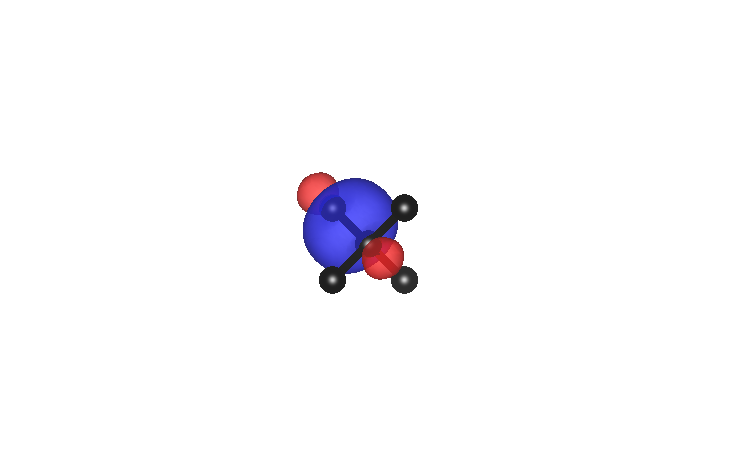
\includegraphics[width=0.2\columnwidth,trim={220pt 120pt 220pt 120pt},clip]{figure/example05/diamond_2.png}}
	\centering
 	\subfloat[\MLWF{} 3]{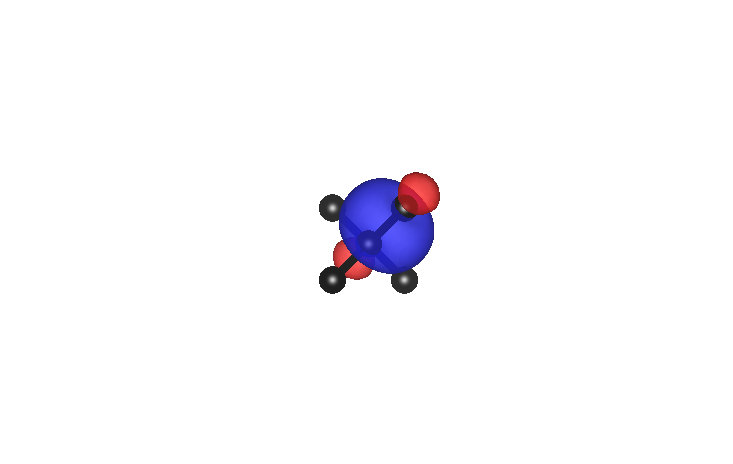
\includegraphics[width=0.2\columnwidth,trim={220pt 120pt 220pt 120pt},clip]{figure/example05/diamond_3.png}}
    \centering
 	\subfloat[\MLWF{} 4]{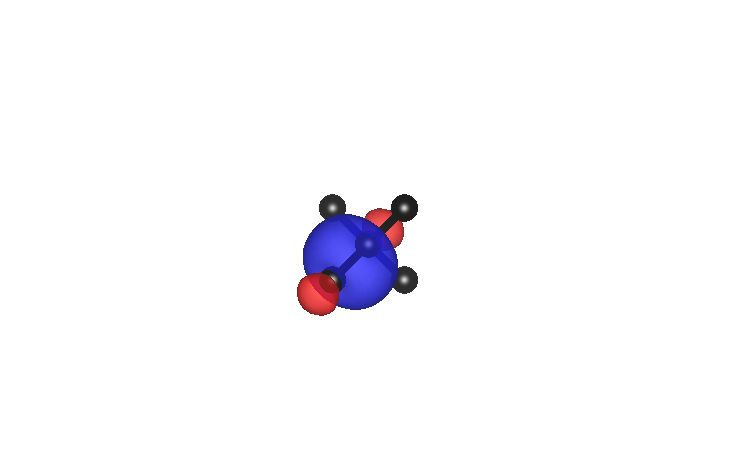
\includegraphics[width=0.2\columnwidth,trim={220pt 120pt 220pt 120pt},clip]{figure/example05/diamond_4.png}}
 	\caption{4 \MLWFs{} in diamond describing the valence bands plotted using \vesta.}\label{fig5.1}
	\end{figure}
